\documentclass[11pt]{article}

\usepackage[T1]{fontenc}
\usepackage[utf8]{inputenc}
\usepackage[english]{babel}
\usepackage{amsmath, amssymb}
\usepackage{graphicx}
\usepackage{booktabs}
\usepackage[margin=2.5cm]{geometry}
\usepackage{csquotes}
\usepackage[hidelinks]{hyperref}

\graphicspath{{figures/}}

\newcommand{\nin}{n^{(i),\mathrm{in}}}
\newcommand{\nbar}{\overline{n}}

\title{Tissue Growth under Large Phenotypic Heterogeneity\\
\large A Finite-Volume Model for Competing Cell Populations}
\author{Joschik Brunow \and Jakob Krautmacher \and Lucas Posern}
\date{Winter term 2025/26}

\begin{document}
\maketitle

\begin{abstract}
\noindent
We simulate the growth of tissue in which several cell types move, divide and
compete for space at the same time. The model follows Dębiec, Mandal and
Schmidtchen (2025): every cell moves along the negative gradient of a shared
pressure (Darcy's law) and grows logistically until the tissue is locally full.
We derive the model, discretize it with a finite-volume scheme, and show
simulations for $N$ species in one dimension and for two species in two
dimensions. In both settings, initially mixed populations separate over time into
spatially distinct regions.
\end{abstract}

\tableofcontents

\section{Introduction}
Simulating how tissue develops helps to predict and understand it, which matters
in tumor research. We present a model that captures several cell types with
different growth properties. In $d$-dimensional space we solve a system of partial
differential equations whose solution is the density of each of the $N$
phenotypes over time $t$.

We first explain the model. We then present an implementation in one dimension for
$N$ species and afterwards show results for two species in two dimensions. Both
implementations solve the system with the finite-volume method.

\section{The mathematical model}
\label{sec:model}
We explain the tissue-growth model of Dębiec, Mandal and Schmidtchen (2025). We
consider $N$ phenotypes and treat time as continuous, then discretize it in the
implementation. We keep the spatial dimension $d \in \mathbb{N}$ general.

\subsection{Pressure and velocity}
We first study how the pressure at different points drives the motion, that is the
velocity and direction. We start from a mass with the same properties everywhere
except for the pressure $p \colon \mathbb{R}^d \to \mathbb{R}$. The motion is a
vector field $v \colon \mathbb{R}^d \to \mathbb{R}^d$ that assigns a direction and
a speed $\lVert v \rVert$ to each point. Darcy's law links the two:
\begin{equation}
    v(x) = -\nabla p(x).
\end{equation}
The negative gradient of $p$ points in the direction of steepest descent and is
orthogonal to the level sets of $p$. The mass therefore moves from the highest
pressure toward the lowest, as expected.

This model stays simplified. It says nothing about how the pressure evolves,
because $v$ and $p$ do not depend on time $t$. We also assume a viscosity $\nu =
0$, so the mass moves without delay. We keep this assumption because it simplifies
both the equations and the implementation.

\subsection{The model for finitely many species}
\subsubsection{Notation}
Let $N \in \mathbb{N}$ be the number of species. We write $n^{(i)}(x, t)$ for the
density of species $i$ at point $x \in \mathbb{R}^d$ and time $t \ge 0$, for each
$i \in \{1, \dots, N\}$. The average density at $x$ and $t$ is
\begin{equation}
    \nbar(x, t) := \frac{1}{N} \sum_{i=1}^{N} n^{(i)}(x, t).
\end{equation}
For brevity we drop the arguments $(x, t)$ from $n^{(i)}$ and $\nbar$.

\subsubsection{Differential equation}
For each phenotype $i \in \{1, \dots, N\}$ the density evolves according to
\begin{equation}
    \frac{\partial n^{(i)}}{\partial t}
    = \nabla \cdot \bigl( n^{(i)} \nabla \nbar \bigr) + n^{(i)} G^{(i)}(\nbar).
    \label{eq:pde}
\end{equation}
The operator $\nabla = \bigl( \tfrac{\partial}{\partial x_1}, \dots,
\tfrac{\partial}{\partial x_d} \bigr)$ collects the $d$ partial derivatives. The
term $\nabla \nbar$ is the overall motion of all cells under Darcy's law.
Multiplied by the density $n^{(i)}$ it gives the actual velocity of species $i$,
and the divergence $\nabla \cdot (n^{(i)} \nabla \nbar)$ states where the density
of that phenotype grows or shrinks.

If no cells are born and none die, the second term vanishes and pure transport
remains:
\begin{equation}
    \partial_t n^{(i)} = \nabla \cdot \bigl( n^{(i)} \nabla \nbar \bigr).
\end{equation}

\subsubsection{The growth rate}
The second term describes the behaviour of the cell types through the growth
function $G^{(i)}$. We define $G^{(i)}$ separately for each phenotype; it depends
on $i$ and on the average density $\nbar \in \mathbb{R}$. Let $G^{(i)} \colon
\mathbb{R}_+ \to \mathbb{R}$, $\nbar \mapsto G^{(i)}(\nbar)$ with the following
properties:
\begin{itemize}
    \item[(G1)] \emph{Continuously differentiable:} $G^{(i)} \in C^1(\mathbb{R})$.
    \item[(G2)] \emph{Strictly decreasing:} $\exists\, \alpha > 0$ with
    $\partial_{\nbar} G^{(i)}(\nbar) \le -\alpha$ for all $\nbar \in \mathbb{R}$.
    \item[(G3)] \emph{Homeostatic pressure:} for each $i$ there is a density
    $n^{\star}_{(i)} > 0$ with $G^{(i)}(n^{\star}_{(i)}) = 0$. We call the largest
    of these values $\nbar^{\star} := \max_{i} n^{\star}_{(i)}$. It depends on
    neither $x$ nor $t$ and is constant for each $i$.
\end{itemize}
The strict monotonicity (G2) reflects that cells divide less easily the higher the
surrounding pressure, since less space remains for new tissue. The homeostatic
pressure (G3) is the point where death and division rates balance. Since
$n^{\star} > 0$, every species grows at a sufficiently small density, and the
monotonicity gives exactly one root. Negative growth turns positive again only
once the pressure has dropped enough.

The growth rate takes the average density $\nbar$ as its argument and is
multiplied by the density of the species at that point. This gives the absolute
amount of growth, which is added to the spatial motion and enters the change in
the density over time.

\subsubsection{Initial condition}
\label{sec:initial}
To simulate the process we need an initial distribution for each phenotype. Let
$\nin \colon \mathbb{R}^d \to [0, \infty)$ be the initial distribution with the
following properties:
\begin{itemize}
    \item[(I1)] \emph{$L^1$ and $L^\infty$ integrability:} $\nin \in
    L^1(\mathbb{R}^d) \cap L^\infty(\mathbb{R}^d)$.
    \item[(I2)] \emph{Boundedness:} $\nin(x) \le \nbar^{\star}$ (see (G3)) for
    Lebesgue-almost every $x \in \mathbb{R}^d$.
    \item[(I3)] \emph{Centrality:} $\int_{\mathbb{R}^d} \nin(x)\, \lVert x
    \rVert^2 \, dx < \infty$.
\end{itemize}
The integral of a density is the total number of cells of that type, so $L^1$
requires finitely many cells. $L^\infty$ bounds the density on every subset of
positive Lebesgue measure, which is also physically reasonable. (I2) tightens this
with the upper bound $\nbar^{\star}$ from (G3): at least one phenotype has a
non-negative growth rate everywhere, so the system does not start overcrowded.
(I3) weights the density by $\lVert x \rVert^2$, so points near the origin count
little and distant points count strongly. A finite integral keeps most cells near
the origin at the start; they spread out later under Darcy's law.

Together with given $G^{(i)}$ and $\nin$, we obtain for all $i \in \{1, \dots,
N\}$ the final system
\begin{equation}
    \begin{aligned}
        \partial_t n^{(i)} &= \nabla \cdot \bigl( n^{(i)} \nabla \nbar \bigr)
        + n^{(i)} G^{(i)}(\nbar), \\
        n^{(i)}(x, 0) &= \nin(x).
    \end{aligned}
\end{equation}

\section{Numerical implementation of the 1D $N$-species model}
\label{sec:1d}
We implement the Darcy model of Section~\ref{sec:model} for finitely many species
in one spatial dimension. The focus is on the discretization, the model
assumptions and the interpretation of the results.

\subsection{A discretization example}
As an illustration we take $d = 1$ with $N = 2$ species on $\Omega = [0, 3]$,
split coarsely into three control volumes of width $\Delta x = 1$:
\[
    C_1 = [0, 1], \quad C_2 = [1, 2], \quad C_3 = [2, 3].
\]
As initial densities we choose the piecewise-constant cell averages
\[
    n^{(1)} = (0.8,\ 0.2,\ 0), \qquad n^{(2)} = (0,\ 0.4,\ 0.6),
\]
which give the average density $\nbar_j = \tfrac{1}{2}\bigl(n^{(1)}_j +
n^{(2)}_j\bigr) = (0.4,\ 0.3,\ 0.3)$. In 1D the velocity field follows from $v =
-\partial_x \nbar$. Discrete differences at the cell faces give
\[
    v_{1 \to 2} \approx -(\nbar_2 - \nbar_1) = 0.1, \qquad v_{2 \to 3} \approx 0.
\]
Mass therefore flows from $C_1$ to $C_2$, while no transport happens between $C_2$
and $C_3$. This shows the pressure balancing from high to low average density.

For the growth we take $G^{(1)}(\nbar) = 1 - \nbar$ and $G^{(2)}(\nbar) = 0.5 -
\nbar$. The local reaction term $n^{(i)}_j G^{(i)}(\nbar_j)$ lets both species grow
where they are present, since $\nbar_j < 1$ and $\nbar_j < 0.5$ in every cell. If
$n^{(i)}_j = 0$, no new species appears. The full dynamics
\[
    \partial_t n^{(i)} = \partial_x\bigl( n^{(i)} \partial_x \nbar \bigr)
    + n^{(i)} G^{(i)}(\nbar)
\]
move existing mass along the gradient of the total density and amplify or damp the
local density depending on the overall occupancy. This minimal example shows the
two central mechanisms: pressure-driven transport from high to low average
density, and growth that $\nbar$ regulates locally. In the next step we treat both
effects together per time step.

\subsection{Discretization and parameters}
The domain is the interval $[0, L]$, divided into $J$ equidistant control volumes
of width $\Delta x = L / J$. The unknowns are the cell densities $n^{i}_j(t)
\approx n_i(x_j, t)$ of the $N$ species at the cell centers $x_j$. We simulate up
to a final time $T$ with a fixed step size $\Delta t$. We choose the pressure as
\begin{equation}
    p(\rho) = \rho^\gamma, \qquad \rho = \sum_{i=1}^{N} n_i,
\end{equation}
where $\gamma > 1$ produces a steeply rising pressure at high total densities. The
species differ only in their constant growth rates $r_i$. For this we discretize
an interval $[r_{\min}, r_{\max}]$ uniformly, permute it at random and assign the
values to the species. This creates heterogeneous but time-constant growth
conditions. As initial data we consider two variants, a strictly separated
distribution and overlapping Gaussian profiles with maxima spread along the
interval. In both cases we scale so that $\rho(x, 0) \le 1$ for all $x$, so the
maximum packing density already holds at the start.

\subsection{Finite-volume scheme}
\label{sec:fv1d}
Each species satisfies
\begin{equation}
    \partial_t n_i + \partial_x (n_i v) = n_i r_i (1 - \rho), \qquad
    v = -\partial_x p(\rho).
\end{equation}
We discretize this equation with an explicit finite-volume scheme. It rests on the
balance over the control volumes and therefore conserves total mass at the
discrete level; Carrillo, Chertock and Huang (2015) give a detailed account. From
the densities we first compute the total density $\rho_j = \sum_i n^{i}_j$ and the
pressure $p_j = (\rho_j)^\gamma$. The velocity at the cell faces then follows from
a discrete derivative,
\begin{equation}
    v_{j + \frac{1}{2}} = -\frac{p_{j+1} - p_j}{\Delta x},
\end{equation}
with no-flux boundary conditions $v_{1/2} = v_{J + 1/2} = 0$. Once the velocity is
known, we discretize the transport with an upwind flux that takes the density from
the upwind cell:
\begin{equation}
    F_{i, j + \frac{1}{2}} =
    \begin{cases}
        v_{j + \frac{1}{2}}\, n^{i}_j,     & v_{j + \frac{1}{2}} \ge 0, \\[4pt]
        v_{j + \frac{1}{2}}\, n^{i}_{j+1}, & v_{j + \frac{1}{2}} < 0.
    \end{cases}
\end{equation}
We set the reaction term locally as $R^{i}_j = n^{i}_j r_i (1 - \rho_j)$; it gives
logistic growth with carrying capacity $\rho = 1$. An explicit time step thus has
four parts: pressure and velocity, fluxes, reaction term, and the density update.
We clip negative values numerically. A sufficiently small $\Delta t$ ensures
stability.

\subsection{Model assumptions}
\label{sec:assumptions1d}
The 1D simulation rests on four assumptions: the tissue is one-dimensional; all
species experience the same pressure field, which depends on the total density;
the local density is bounded by $\rho \le 1$; and we use insulating boundary
conditions. Section~\ref{sec:overview} gives a full overview of all assumptions of
the model and both implementations.

\subsection{Visualization and phase separation}
For selected times we show two views: the absolute density of one species together
with the total density, and the relative fraction of one species in the total
population.

\paragraph{Case 1: strictly separated initial distribution.}
Two species start in disjoint regions, so competition first occurs only at the
interface. The species with the higher growth rate builds up more local pressure
and displaces the slower one. After the total density reaches its maximum, a
stable, spatially separated configuration sets in (Figure~\ref{fig:case1}).

\begin{figure}[htbp]
    \centering
    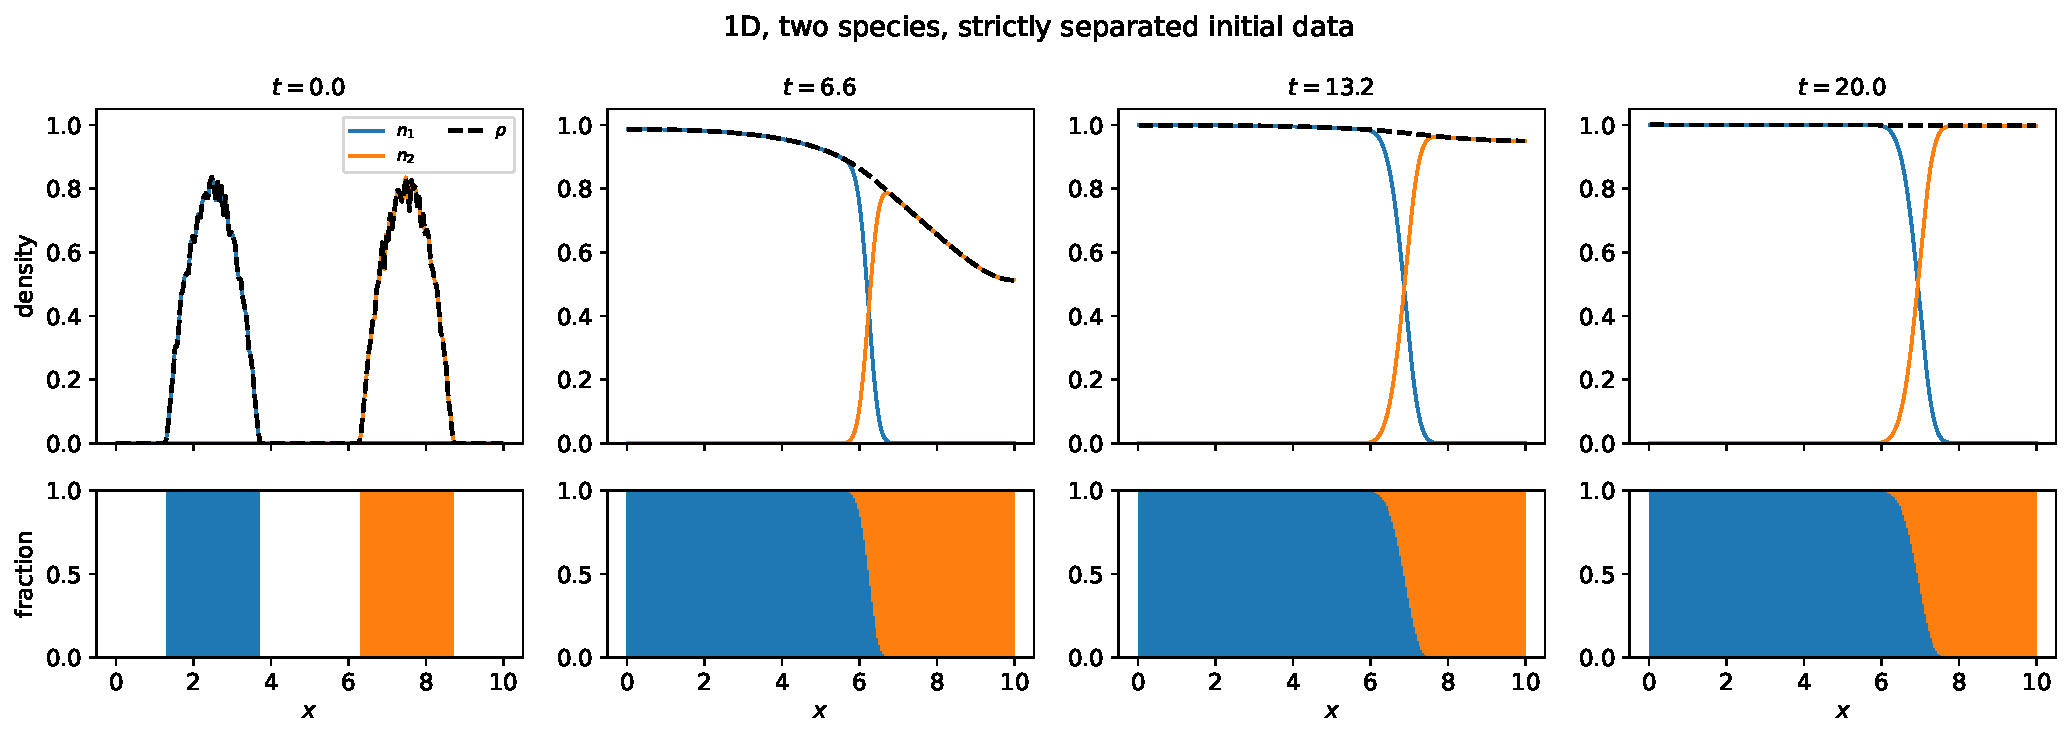
\includegraphics[width=\textwidth]{fig_1d_separated.pdf}
    \caption{Case 1: evolution of the cell distribution for a strictly separated
    initial distribution.}
    \label{fig:case1}
\end{figure}

\paragraph{Case 2: overlapping Gaussian profiles.}
Several species start with overlapping Gaussian profiles and therefore in direct
competition. In the same spatial regions, faster-growing species reach higher
densities and displace slower ones. Over time a clear phase separation into
distinct domains emerges, while the total density reaches the bound $\rho = 1$
(Figure~\ref{fig:case2}).

\begin{figure}[htbp]
    \centering
    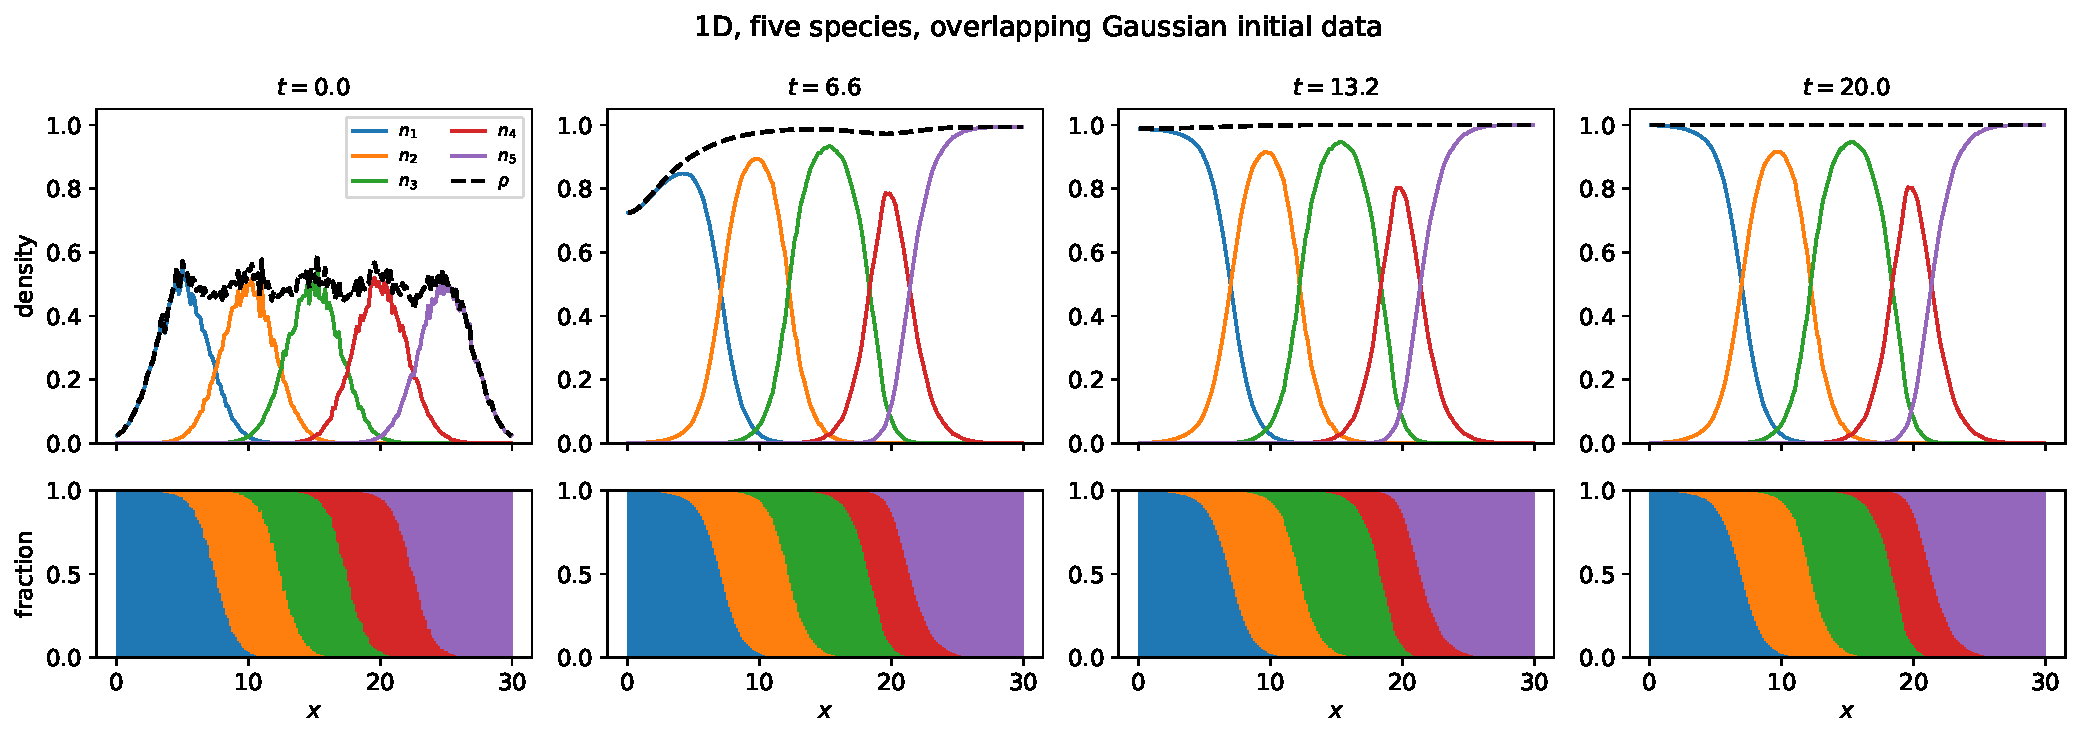
\includegraphics[width=\textwidth]{fig_1d_gaussian.pdf}
    \caption{Case 2: evolution of the cell distribution for overlapping Gaussian
    bells.}
    \label{fig:case2}
\end{figure}

\section{Numerical implementation of the 2D two-species model}
\label{sec:2d}

\subsection{Structure and parameters}
We implement the simulation in Python as the class \texttt{TissueSim2D}. All
attributes can be changed and all methods called flexibly, which eases parameter
studies and extensions. The class provides the following methods:
\begin{itemize}
    \item \texttt{\_\_init\_\_}: initializes the grid, the model parameters and the
    initial densities.
    \item \texttt{update\_n}: computes the new densities from those of the previous
    step with a finite-volume scheme and explicit Euler.
    \item \texttt{run}: runs the simulation over all steps and stores snapshots at
    regular intervals.
    \item \texttt{visualize}: shows both species, the total density and a direct
    comparison.
    \item \texttt{save} / \texttt{load}: store or load the full simulation state.
\end{itemize}

The main parameters are the grid size \texttt{grid\_size} (the grid has
\texttt{grid\_size} $\times$ \texttt{grid\_size} cell-centered control volumes),
the number of steps \texttt{count\_timesteps}, the step size \texttt{dt}, the
snapshot interval \texttt{snapshot\_every} and the boundary type
\texttt{boundary} (\texttt{neumann} or \texttt{dirichlet}). The species behaviour
is set by the growth rates \texttt{G1}, \texttt{G2}, the competition coefficients
\texttt{comp1}, \texttt{comp2} (growth inhibition by the other species), the
pressure response \texttt{beta1}, \texttt{beta2} and the self-diffusion
\texttt{eps1}, \texttt{eps2}. The initial distribution is fixed by \texttt{center},
\texttt{peak}, \texttt{sigma} and \texttt{background} for both species. The default
parameters are symmetric, so the influence of a single parameter can be studied in
isolation.

\subsection{Finite-volume scheme and time discretization}
\subsubsection{Equations}
The model consists of two coupled conservation laws for $i, j \in \{1, 2\}$ with
$i \neq j$:
\begin{equation}
    \partial_t n_i + \nabla \cdot (n_i v_i) = \varepsilon_i \Delta n_i
    + G_i\, n_i (1 - n_i - c_i n_j), \qquad
    v_i = -\beta_i \nabla \nbar, \quad \nbar = \tfrac{1}{2}(n_1 + n_2).
\end{equation}
Compared with the 1D model, two effects are added: the self-diffusion
$\varepsilon_i \Delta n_i$ and the asymmetric competition through the coefficients
$c_i$.

\subsubsection{Spatial discretization}
The densities $n^{k,l}_i$ are cell-centered averages on a uniform grid with $0 \le
k, l \le N - 1$; we evaluate the fluxes at the faces $k \pm \tfrac{1}{2}, l$ and
$k, l \pm \tfrac{1}{2}$. We first approximate the face velocities with finite
differences,
\begin{equation}
    v^{k + \frac{1}{2}, l}_{i, x} = -\beta_i \frac{n^{k+1, l} - n^{k, l}}{\Delta x},
    \qquad
    v^{k, l + \frac{1}{2}}_{i, y} = -\beta_i \frac{n^{k, l+1} - n^{k, l}}{\Delta y}.
\end{equation}
From these we form the advective flux $F = v n$ with the density taken upwind,
\begin{equation}
    F^{k + \frac{1}{2}, l}_x =
    \begin{cases}
        v^{k + \frac{1}{2}, l}_x\, n^{k, l},   & v_x \ge 0, \\[3pt]
        v^{k + \frac{1}{2}, l}_x\, n^{k+1, l}, & v_x < 0,
    \end{cases}
    \qquad
    F^{k, l + \frac{1}{2}}_y =
    \begin{cases}
        v^{k, l + \frac{1}{2}}_y\, n^{k, l},   & v_y \ge 0, \\[3pt]
        v^{k, l + \frac{1}{2}}_y\, n^{k, l+1}, & v_y < 0.
    \end{cases}
\end{equation}
The divergence follows from the difference of the face fluxes,
\begin{equation}
    (\nabla \cdot F)^{k, l}
    = \frac{F^{k + \frac{1}{2}, l}_x - F^{k - \frac{1}{2}, l}_x}{\Delta x}
    + \frac{F^{k, l + \frac{1}{2}}_y - F^{k, l - \frac{1}{2}}_y}{\Delta y}.
\end{equation}
The local growth term is $R^{k, l}_i = G_i\, n^{k, l}_i \bigl(1 - n^{k, l}_i - c_i
n^{k, l}_j\bigr)$.

\subsubsection{Time discretization and stability}
Once the flux divergence and the reaction term are known, we integrate with an
explicit Euler scheme:
\begin{equation}
    n^{k, l}_i(t + \Delta t) = n^{k, l}_i(t) + \Delta t \Bigl(
    -(\nabla \cdot F_i)^{k, l} + \varepsilon_i (\Delta n_i)^{k, l} + R^{k, l}_i
    \Bigr).
\end{equation}
The explicit scheme is subject to stability limits, a CFL condition for the
advection and a diffusion condition of the form $\Delta t \lesssim C \Delta x^2 /
\varepsilon_i$. We choose $\Delta t$ empirically so that the solutions stay stable
in the parameter ranges considered; we do not carry out a formal stability
analysis.

\subsubsection{Boundary conditions}
We treat the boundary in two ways. The Neumann condition extends the boundary
values by first-order constant extrapolation from the interior, so the normal flux
vanishes and total mass is conserved. The Dirichlet condition sets all boundary
cells to zero after each step and models a hostile environment in which cells at
the boundary are removed immediately.

\subsection{Visualization of the results}
The visualization shows four heatmaps: the density of the first species, that of
the second, the total density and a direct comparison. A slider sets the time, and
a checkbox toggles the contours. Red stands for species~1, blue for species~2.

\paragraph{Default run and variations.}
Starting from the same initial state, we change individual parameters. A higher
growth rate ($\texttt{G1} = 1.3$) lets species~1 spread faster and displace
species~2. A stronger pressure response ($\texttt{beta1} = 3.0$) moves species~1
noticeably faster than species~2. Changing several parameters at once lets us
compare very different cell types and observe their behaviour in the model.

\begin{figure}[htbp]
    \centering
    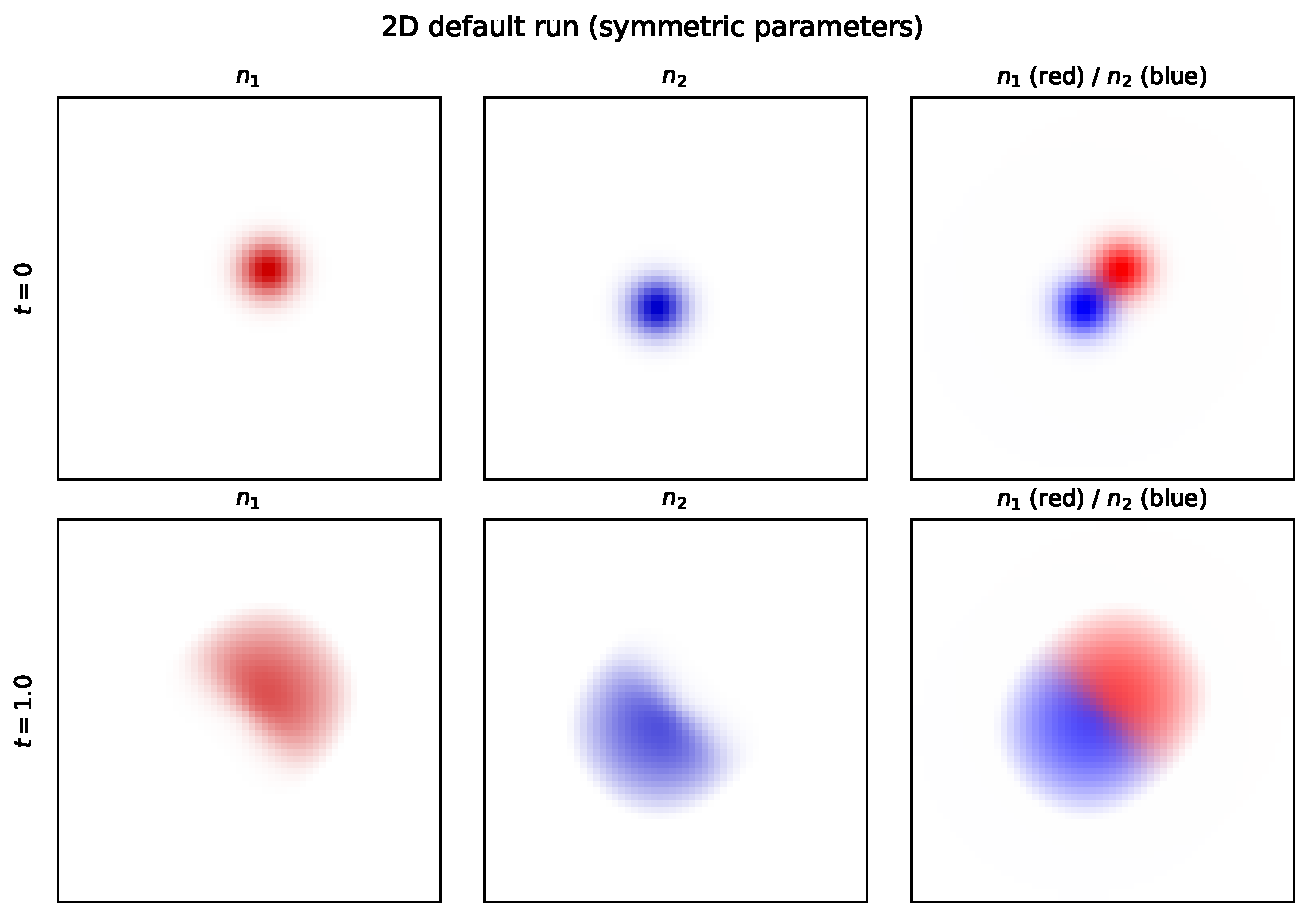
\includegraphics[width=\textwidth]{fig_2d_default.pdf}
    \caption{Default run with symmetric parameters: initial and developed state.
    Red is species~1, blue is species~2.}
    \label{fig:2d_default}
\end{figure}

\begin{figure}[htbp]
    \centering
    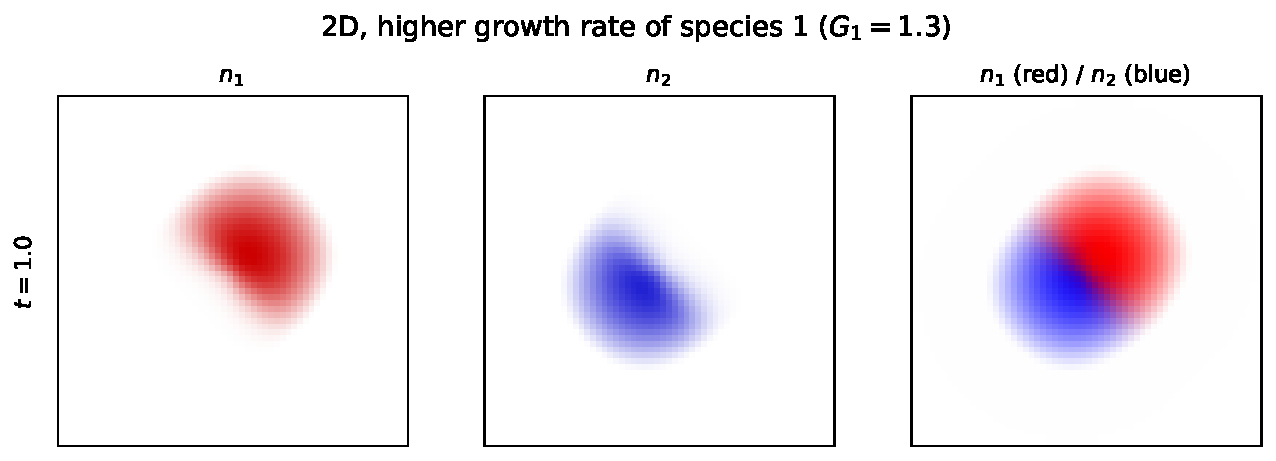
\includegraphics[width=0.92\textwidth]{fig_2d_growth.pdf}
    \caption{Higher growth rate of species~1 ($G_1 = 1.3$): species~1 grows
    faster and displaces species~2 more.}
    \label{fig:2d_growth}
\end{figure}

\begin{figure}[htbp]
    \centering
    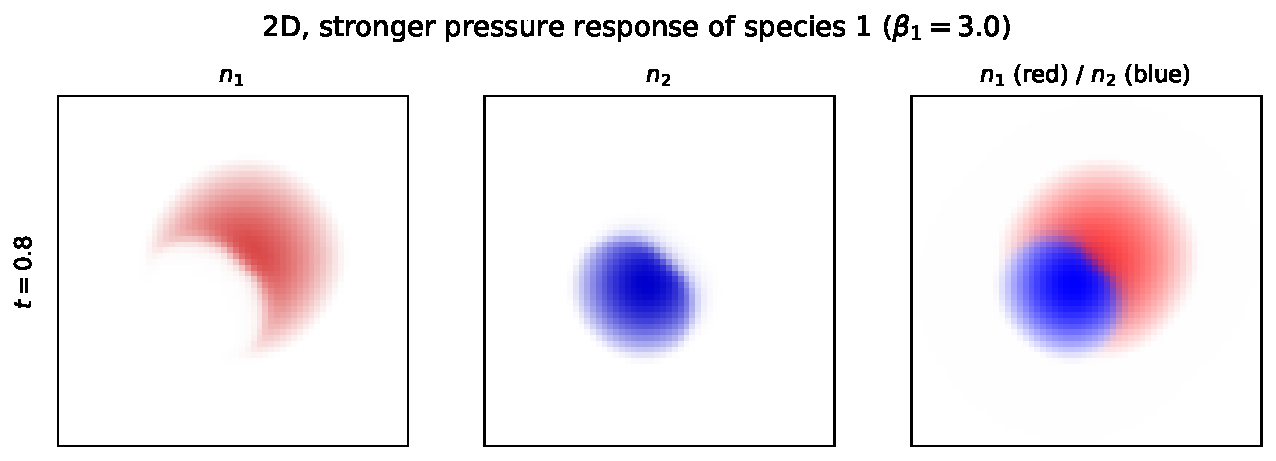
\includegraphics[width=0.92\textwidth]{fig_2d_pressure.pdf}
    \caption{Stronger pressure response of species~1 ($\beta_1 = 3.0$):
    species~1 spreads out much faster than species~2.}
    \label{fig:2d_pressure}
\end{figure}

\section{Overview of all assumptions}
\label{sec:overview}
Table~\ref{tab:assumptions} summarizes the assumptions on which the model and its
two implementations rest.

\begin{table}[htbp]
    \centering
    \begin{tabular}{@{}p{4.2cm}p{10.3cm}@{}}
        \toprule
        \textbf{Area} & \textbf{Assumption} \\
        \midrule
        Motion (Darcy) & Velocity $v = -\nabla p$; viscosity $\nu = 0$, so motion
        is instantaneous. \\
        Pressure & Shared pressure field $p(\rho) = \rho^\gamma$ with $\gamma > 1$,
        depending only on the total density $\rho$. \\
        Growth (G1--G3) & $G^{(i)} \in C^1$, strictly decreasing
        ($\partial_{\nbar} G^{(i)} \le -\alpha$), with a single homeostatic
        pressure $n^{\star}_{(i)} > 0$. \\
        Initial data (I1--I3) & $\nin \in L^1 \cap L^\infty$, bounded by
        $\nbar^{\star}$, with a finite second moment (central initial
        distribution). \\
        Saturation & Maximum local density $\rho \le 1$, already satisfied at the
        start. \\
        Geometry & 1D model on $[0, L]$ or 2D model on the unit square. \\
        Boundary & Insulating (Neumann) conditions; Dirichlet as an alternative in
        2D. \\
        Time & Explicit Euler; $\Delta t$ chosen empirically below the CFL and
        diffusion limits. \\
        2D addition & Self-diffusion $\varepsilon_i \Delta n_i$ and asymmetric
        competition $c_i$ between the two species. \\
        \bottomrule
    \end{tabular}
    \caption{Overview of the model and implementation assumptions.}
    \label{tab:assumptions}
\end{table}

\begin{thebibliography}{9}
\bibitem{carrillo2015}
J.~A. Carrillo, A.~Chertock, and Y.~Huang.
\newblock A finite-volume method for nonlinear nonlocal equations with a gradient
flow structure.
\newblock \emph{Communications in Computational Physics}, 17(1):233--258, 2015.

\bibitem{debiec2025}
T.~Dębiec, M.~Mandal, and M.~Schmidtchen.
\newblock From finite to continuous phenotypes in (visco-)elastic tissue growth
models.
\newblock \emph{Journal of Differential Equations}, 437:113375, 2025.
\end{thebibliography}

\end{document}
